\documentclass[runningheads,a4paper]{llncs}

\usepackage{amssymb}
\usepackage{graphicx}

\usepackage{amsmath, amssymb}

\usepackage{pgfplots}
\usepackage{subfig}
\usepackage[hidelinks]{hyperref}
\def\UrlBreaks{\do\/\do-}
\usepackage{url}
\usetikzlibrary{arrows,calc}
\pgfplotsset{width=3.4cm,compat=1.7}

\renewcommand{\UrlFont}{\footnotesize}
\usepackage{listings, color}


\authorrunning{Ran Wei, John Clark}


\definecolor{mygray}{rgb}{0.95,0.95,0.95}
\lstset{frame=none,
	backgroundcolor=\color{mygray},
	language=Octave,
	aboveskip=3mm,
	belowskip=3mm,
	showstringspaces=false,
	columns=flexible,
	basicstyle={\small\ttfamily},
	xleftmargin=15pt,
	numbers=left,
	breaklines=true,
	breakatwhitespace=false,
	tabsize=2,
	captionpos=b,
}

\begin{document}
	
	\title{\textbf{{Probabilistic Smoothing of Genetic Programming}}}
	\author{Ran Wei \and John A. Clark}
	\institute{Department of Computer Science, \\ University of York, United Kingdom \\ ran.wei, john.clark@york.ac.uk}
	\maketitle
	
	\begin{abstract}
Conventional genetic programming involves the 
\end{abstract}
	
	\section{Introduction}
	\section{Background and Motivation}
	\section{Symbolic Regression: Deterministic}
At first we discuss a case study which is an extended version of the multivalued symbolic regression problem provided as an tutorial for ECJ (Evolutionary Computation in Java)\footnote{\url{https://cs.gmu.edu/~eclab/projects/ecj/docs/tutorials/tutorial4/index.html}}. 

\subsection{Representation}
In the symbolic regression problem, there are six nodes representing the terminals nodes \textbf{X} and \textbf{Y}, and the function nodes \textbf{add} (+), \textbf{sub} (-), \textbf{mul} (*), and \textbf{div} (/). 
\begin{figure}
	\centering
	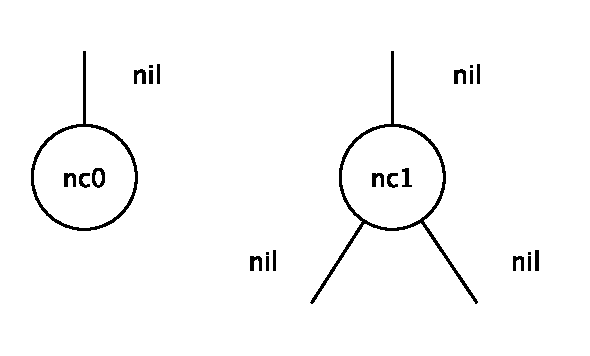
\includegraphics[width=0.5\linewidth]{./fig/symbolic_example_ncs}
	\caption{Node constraints for the symbolic regression problem.}
	\label{fig:symb_ncs}
\end{figure}

The terminal nodes conform to the node constraint \emph{nc0}, and the function nodes conform to the node constraint \emph{nc1} in Figure~\ref{fig:symb_ncs}. \emph{nc0} specifies that nodes which conform to it (Nodes \textbf{X} and \textbf{Y}) should have their return types as \emph{nil}, which is ECJ's default type. \emph{nc0} nodes should have 0 children. \emph{nc1} specifies that the nodes which conform to it (Nodes \textbf{add}, \textbf{sub}, \textbf{mul}, and \textbf{div}) should have their return types as \emph{nil}, \emph{nc1} nodes should have two children, for which their return type should also be \emph{nil}. The function \textbf{div} is added atop the example provided by ECJ and needs additional handling which will be discussed later. 

\subsection{Fitness}
The objective of the symbolic regression is to evolve an equation which satisfies a set of $(X, Y, f(X, Y))$ data. In the current implementation, an upfront equation is provided: $x^2y + xy + y$. For each tree, the evaluation proceeds by giving each \textbf{X} and \textbf{Y} 20 random values and calculating their expected results (denoted by \emph{ev}). Then, the tree generated by GP is evaluated (of which value is denoted by \emph{v}). The \emph{fitness} of the current generation is the sum of the the difference between \emph{ev} and \emph{v}. The optimal would be an equation which is equivalent to $x^2y + xy + y$. The introduction of the \textbf{div} function introduces the possibility of division by 0. To handle such situations, the \emph{fitness} of the tree is set to the maximum value if a division by 0 is detected, such that a tree which contains division by zero is discarded very early in the evolution process. 

We observe that the global optimal is obtained within 20 generations of evolution. 
	\section{Symbolic Regression: Our Approach}
	
	\section{The Occupancy Classification Problem: Deterministic}

In this section we adapt our approach to the study of the classification problem presented in \cite{Candanedo201628}. In this study, data collected from sensors in a room, such as temperature, humidity, light, and $CO_2$ levels (and other fields derived from the aforementioned) are used to determine if the room is occupied. The data and the occupancy are used to train the classification models. In this section, we first present the classification model we implemented using ECJ, we then adapt our approach to the classification problem and evaluate our hypothesis.

\subsection{Representation}
In order for our approach to apply, we first represent the problem using ECJ with only deterministic nodes. 

In the occupancy classification problem, there are eight different types of data that are used in the study: \emph{temperature}, \emph{humidity}, \emph{light}, $CO_2$, \emph{humidity ratio}, \emph{number of seconds from midnight} (denoted by \emph{nsm}), week status (denoted by \emph{ws}) and \emph{occupancy}. In our representation, there are seven terminal nodes \textbf{T} (temperature), \textbf{H} (humidity), \textbf{L} (light), \textbf{HR} (humidity ratio), \textbf{NSM} (number of seconds from midnight) and \textbf{WS} (week status). There are also four function nodes \textbf{add} (+), \textbf{sub} (-), \textbf{mul} (*), and \textbf{div} (/). 

The node constraints are the same as it is illustrated in Figure~\ref{fig:symb_ncs}, where nodes \textbf{T}, \textbf{H}, \textbf{L}, \textbf{HR}, \textbf{NSM} and \textbf{WS} conform to \emph{nc0} and nodes \textbf{add}, \textbf{sub}, \textbf{mul}, and \textbf{div} conform to \emph{nc1}.

\subsection{Fitness}

The objective of the classification problem is to determine if a room is occupied with the data. In our implementation we use an threshold approach. In the training data provided\footnote{\url{https://archive.ics.uci.edu/ml/datasets/Occupancy+Detection+}}, there are 8143 data entries. We obtained the threshold (denoted by $\theta$) by summing the means of all types of data:
\begin{align*}
\theta = \overline{T} + \overline{H} + \overline{L} + \overline{HR} + \overline{NSM} + \overline{WS}
\end{align*}
When the evaluated value of a tree (denoted by \emph{v}) is obtained, we compare \emph{v} with the threshold $\theta$ to form our functional cost ($cost_f$):
\begin{align*}
v \leq \theta \Rightarrow cost_f = 1;\\
v > \theta \Rightarrow cost_f = 0;
\end{align*}

In order to guarantee that all seven terminals are used, we check for existence of the terminals regardless of repetitions (denoted as the parameter cost $cost_{param}$). If all seven terminals are used, $cost_{param}$ is 0, otherwise $cost_{param}$ equals the number of terminals that are not used. 

We then define our fitness:
\begin{align*}
fitness = cost_f + cost_{param}
\end{align*}

With our implementation we managed to get 98.99\% accuracy within 30 generations of evolution in ECJ. However, the accuracy is not able to improve any further.

\section{The Occupancy Classification Problem: Stochastic}

%An abstract representation of our initial classification model is illustrated in Figure \ref{fig:class_abstract-tree} to better understand our approach. The representation contains a number of functions (in this case study, $<$, $>$, $\leq$ and $\geq$) and a number of terminals (\emph{1} and \emph{0} representing if a room is occupied or not). When the tree is evaluated, data from a single data set (the set containing the data from all the sensors at a specific point in time) is selected and used to determine if a room is occupied. In our implementation, an ideal classification model is \emph{searched} using the data provided in the study \cite{}. The types of data used in our implementation are \emph{temperature}, \emph{humidity}, \emph{light}, \emph{co2}, \emph{humidity ratio}, \emph{NSM} (the number of seconds from midnight for each day) and \emph{WS} (week status, derived from the time stamp provided, which yields 1 if weekdays and 0 otherwise).
%
%The function nodes in our implementation has a number of attributes:
%\begin{itemize}
%	\item A data type to compare. With the data type, the node is able to select the data by its type from the data set provided.
%	\item A value to compare with the actual data of the data type. For example the root node in Figure \ref{fig:class_abstract-tree} compares the light level (actual data) with a value (365). This value is likely to be determined by trial or automatically by evolution.
%	\item Two child nodes which can be either terminals or function nodes. In our implementation, child 0 (the child on the left) always represent the \emph{false} value, so that when the result of the evaluation is false, the evaluation goes to child 0. The sample principle applies to child 1. It is to be noted that if a terminal is reached, the evaluation of the whole tree is completed, and the evaluation result is whatever value of the terminal.
%\end{itemize}
%
%Based on the abstract representation, we implement our representation of the classification problem in ECJ. 
%
%\subsubsection{Atomic Types and Set Types}
%In our implementation, there are four atomic types, \emph{nil}, \emph{bool}, \emph{data} and \emph{int}. There is also a set type, \emph{nil-or-bool}. In ECJ, this means that when an edge is declared to accept \emph{nil-or-bool}, it accepts nodes that return either \emph{nil} or \emph{bool}. The usage of atomic types and the set type will be discussed later.
%
%\subsubsection{Node Constraints for Terminals}
%In our implementation, three node constraints for terminals have been defined, which are shown in Figure \ref{fig:class-terminals}. \emph{nc0}, \emph{nc1} and \emph{nc2} respectively defines that for these types of terminals, their return types should be \emph{bool}, \emph{data} and \emph{int} respectively.
%
%%\begin{figure}[ht!]
%%	\centering
%%	\includegraphics[width=1\linewidth]{./fig/class_terminals}
%%	\caption{Terminals used in the classification problem}
%%	\label{fig:class-terminals}
%%\end{figure}
%
%\subsubsection{Terminals}
%With the node constraints, we define 11 terminal nodes in the function set.
%\begin{itemize}
%	\item Terminals \emph{Result\_Zero} and \emph{Result\_One} with node constraint \emph{nc0}. These two nodes represent the boolean values 1 and 0 where 1 represents true and 0 represents false. 
%	\item Terminals \emph{Temperature}, \emph{Humidity}, \emph{Light}, \emph{CO2}, \emph{HumidityRatio}, \emph{NSM} and \emph{WS} with node constraint \emph{nc1}. These terminals are used to extract the data from the classification problem. 
%	\item Terminals \emph{Numeral\_Zero} and \emph{Numeral\_One} which represent integer values 1 and 0, which are used to denote a binary digit (bit).
%\end{itemize}
%
%\subsubsection{Node Constraints for Non-Terminals}
%One node constraint (named \emph{nc4}) is defined for the non-terminals used in our implementation, which is shown in Figure \ref{fig:class-non-terminals}. The constraints are:
%%\begin{figure}
%%	\centering
%%	\includegraphics[width=0.8\linewidth]{./fig/class_non-terminal}
%%	\caption{Terminals used in the classification problem}
%%	\label{fig:class-non-terminals}
%%\end{figure}
%\begin{itemize}
%	\item The return type of the node is \emph{nil}. 
%	\item The children at index 0 and index 1 (ordered specifically in this way) accepts set type \emph{nil-or-bool}. This means that the return types of the child nodes can be either \emph{nil} (in this instance only the nodes that conform to \emph{nc4}) or \emph{bool} (the nodes that conform to \emph{nc0}).
%	\item Child(2) to child(26) are used to compute the \emph{value} of the node. These children can only be terminals that conform to \emph{nc2}. The \emph{value} as previously mentioned, is used to compare with the actual data of the node of a certain type (temperature, humidity, etc.). The value $v$ is formed of a decimal part and a fraction part. Child(2) to child(18) are used to derive the decimal part (denoted as $d$), each child represents a bit in place, with a total number of 17 bits. The reason for this is because that the data type \emph{NSM} can get up to 86399 (seconds in a day). Child(19) to child(22) (4 bits) are used to derive a number (denoted by $f1$) and then used to derive a numerator (denoted by $fn$) which is calculated by repeatedly dividing $f1$ by 10 until it is less than 1. Child(23) to child(26) (4 bits) are used to derive another number (denoted by $f2$), this number is then convert to a denominator (denoted by $fd$) where  
%	\begin{align*}
%		fd = 10^{f2}
%	\end{align*}
%	Thus, the value $v$ is calculated as such:
%	\begin{align*}
%		v = d + fn/fd
%	\end{align*}
%	In this sense, $v$ covers at least the granularity of the possible numbers that may be used to compare with the actual data in this case study.
%	\item Child[27] is used to extract the data from the classification problem. This child can only be terminals that conform to \emph{nc1}. 
%\end{itemize}
%
%\subsubsection{Non Terminals}
%With the node constraints, we define 4 non-terminal nodes in the function set:
%\begin{itemize}
%	\item \emph{GreaterThan}
%	\item \emph{GreaterThanOrEqualTo}
%	\item \emph{LessThan}
%	\item \emph{LessThanOrEqualTo}
%\end{itemize} 
%For each node, it selects a data type and its associated data first, it then generates the \emph{value} to be compared aforementioned, and then finally, the operator ($<$, $>$, $\leq$ and $\geq$) are used to compare these values. If the evaluation is true, the child at index 1 is evaluated. If the evaluation is false, the child at index 0 is evaluated. The evaluation of the tree completes when a terminal is reached throughout the evaluation.
%
%\subsubsection{Tree Constraint}
%The tree constraint is default for ECJ where the tree return type is \emph{nil}, this guarantees that the root of a tree can only be a non-terminal node that conforms to \emph{nc4}
%
%

	

	\bibliographystyle{unsrt} 
	\bibliography{paper1}  
	
\end{document}
